% Compile twice with pdflatex.
% Paper: Ahlfeldt, Redding, Sturm and Wolf (2015), Econometrica 83(6).
\pdfminorversion=7
\documentclass[aspectratio=169,11pt]{beamer}
\usetheme{default}
\usecolortheme{default}
\usefonttheme{professionalfonts}
\usepackage[T1]{fontenc}
\usepackage{lmodern}
\usepackage{amsmath,amssymb,booktabs,graphicx,array}
\usepackage{tikz}
\usetikzlibrary{arrows.meta}
\definecolor{navy}{RGB}{0,45,98}
\definecolor{accent}{RGB}{200,90,25}
\definecolor{lightgrey}{RGB}{242,242,242}
\colorlet{CIEdark}{navy}
\colorlet{CIEorange}{accent}
\colorlet{CIEgrey}{black!65}
\setbeamercolor{frametitle}{fg=navy}
\setbeamercolor{title}{fg=navy}
\setbeamercolor{structure}{fg=navy}
\setbeamercolor{alerted text}{fg=accent}
\setbeamerfont{frametitle}{series=\bfseries,size=\Large}
\setbeamertemplate{navigation symbols}{}
\setbeamertemplate{itemize items}[circle]
\setbeamertemplate{footline}{%
  \hfill\usebeamercolor[fg]{structure}\scriptsize
  \insertshortauthor\quad\insertframenumber/\inserttotalframenumber
  \hspace{1em}\vspace{0.8em}}
\setbeamersize{text margin left=0.8cm,text margin right=0.8cm}
\newcommand{\tightitems}{\setlength{\itemsep}{0.55em}}
\newcommand{\smallgap}{\vspace{0.35em}}

\title{The Economics of Density}
\subtitle{Evidence from the Berlin Wall\\[0.5em]
  \small Ahlfeldt, Redding, Sturm and Wolf (2015)}
\author[Dominic Behrens]{Dominic Behrens}
\institute{The Centre for International Economics}
\date{21 October 2026}


\newcommand{\decksection}[1]{%
  \section{#1}
  \begin{frame}[plain]
    \vfill{\usebeamerfont{title}\color{navy}\LARGE #1}\vfill
  \end{frame}}
\tikzset{term/.style={font=\Large,inner sep=2pt},
  lab/.style={font=\small,text=navy,align=center},
  arr/.style={-{Stealth[length=1.8mm]},accent,thick}}


\begin{document}
\begin{frame}[plain]
  \titlepage
\end{frame}
\decksection{Motivation and Background}
\begin{frame}{Models of Cities}
  \begin{itemize}\setlength{\itemsep}{1.2em}
    \item Your friend and mine, the Alonso--Muth--Mills model: monocentric city, bid-ask gradients, lots of fun, way too abstracted to make precise predictions. 
    \item Some extensions: assorted Fujita \& Krugman throughout the 90s, Lucas \& Rossi-Hansberg (2003) give more flexibility in firm location and allow for agglomeration and location-varying productivity but only on a simple disk  
  \end{itemize}
\end{frame}
\begin{frame}{Issues with These Models}
  These models do not capture important features of cities:
  \vspace{0.7em}
  \begin{itemize}\setlength{\itemsep}{1.0em}
    \item Real-world, non-radial transport networks
    \item Local amenities and production externalities for residents
    \item Dispersed employment across cities
  \end{itemize}
\end{frame}
\begin{frame}{Contributions of This Paper}
  \begin{itemize}\setlength{\itemsep}{1.2em}
    \item A tractable quantitative spatial model (QSM) for counterfactuals
      and policy analysis.
    \item Estimates of agglomeration externalities and other highly important parameters 
    \item CRAZY data work
  \end{itemize}
\end{frame}
% Historical context: Ahlfeldt et al. (2015), Section 2.
\begin{frame}{The Berlin Wall: Timeline}
  \begin{columns}[c,onlytextwidth]
    \begin{column}{0.46\textwidth}
      \begin{itemize}\setlength{\itemsep}{1.0em}
        \item \textbf{1945--1949:} Berlin divided, separate East and West German states established in 1949.
        \item \textbf{1961:} East Germany closes the border and builds the wall, ending commuting between East and West Berlin.
        \item \textbf{1989:} The wall comes down.
      \end{itemize}
    \end{column}
    \begin{column}{0.50\textwidth}
      \centering
      % Photograph: J Dykstra, 1988; released into the public domain.
      % https://commons.wikimedia.org/wiki/File:Berlin_wall_1988.jpg
      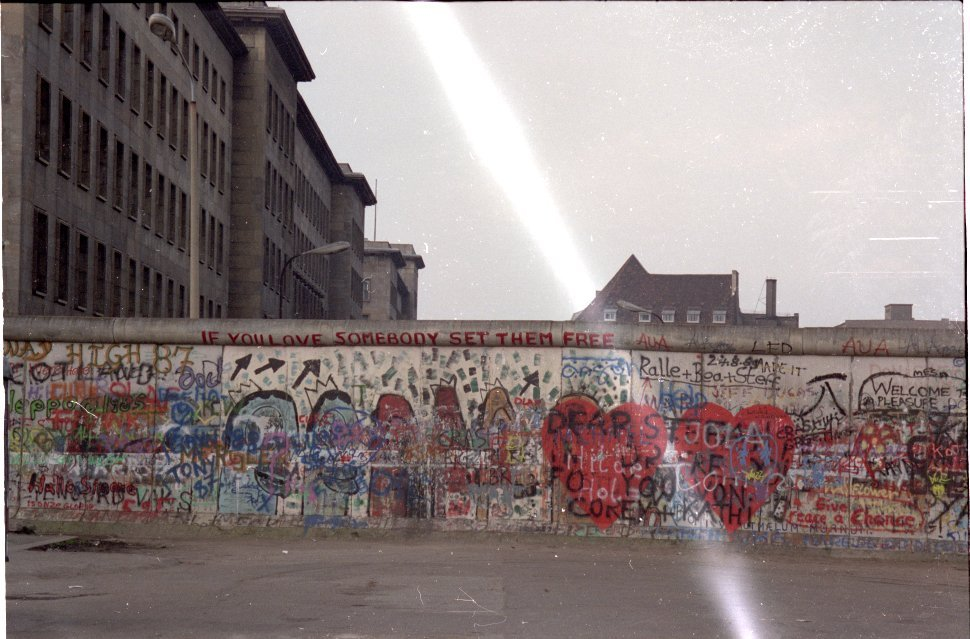
\includegraphics[width=\linewidth]{figures/berlin-wall-1988.jpg}
    \end{column}
  \end{columns}
\end{frame}
\decksection{Data}
\begin{frame}{Land Prices in Berlin, 1936}
  \centering
  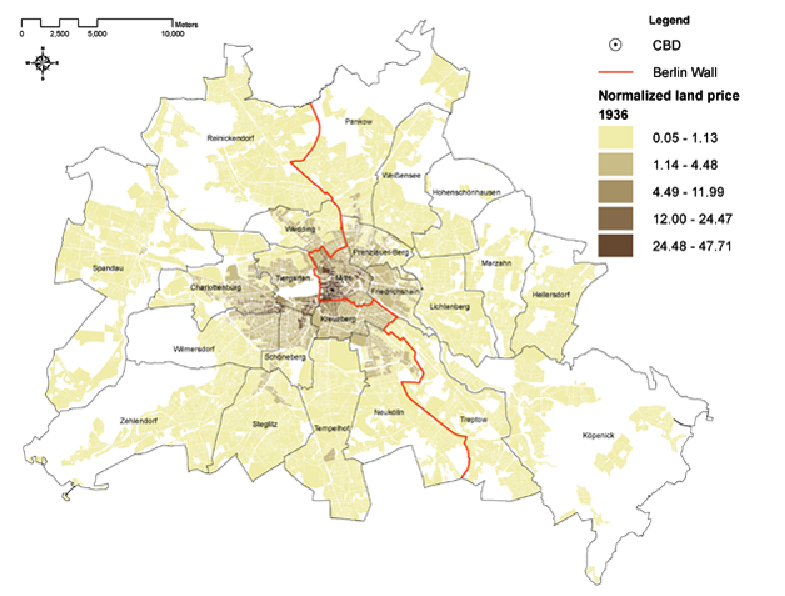
\includegraphics[width=\textwidth,height=0.77\textheight,keepaspectratio]{figures/berlin-1936.pdf}
\end{frame}

\begin{frame}{Land Prices: Berlin, 1936}

  \centering
  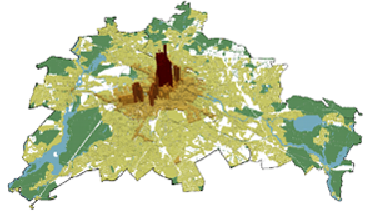
\includegraphics[width=0.88\textwidth,height=0.77\textheight,keepaspectratio]{figures/figure2-a.pdf}
\end{frame}

\begin{frame}{Land Prices: West Berlin, 1936}

  \centering
  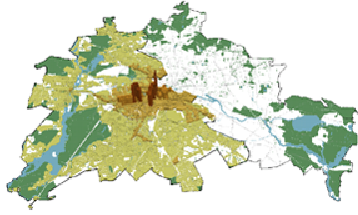
\includegraphics[width=0.88\textwidth,height=0.77\textheight,keepaspectratio]{figures/figure2-b.pdf}
\end{frame}

\begin{frame}{Land Prices: West Berlin, 1986}

  \centering
  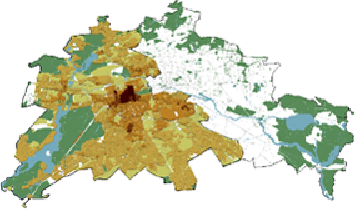
\includegraphics[width=0.88\textwidth,height=0.77\textheight,keepaspectratio]{figures/figure2-c.pdf}
\end{frame}

\begin{frame}{Land Prices: Berlin, 2006}

  \centering
  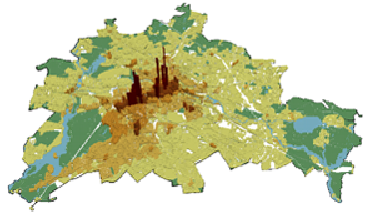
\includegraphics[width=0.88\textwidth,height=0.77\textheight,keepaspectratio]{figures/figure2-d.pdf}
\end{frame}

\begin{frame}{Land Prices: West Berlin, 2006}

  \centering
  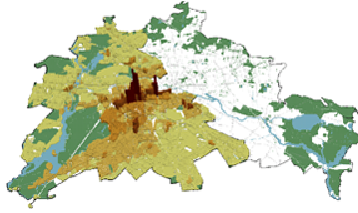
\includegraphics[width=0.88\textwidth,height=0.77\textheight,keepaspectratio]{figures/figure2-e.pdf}
\end{frame}


% Data definitions and sources: Ahlfeldt et al. (2015), Section 4.
\begin{frame}{Other Key Data Sources}
  \begin{itemize}\setlength{\itemsep}{0.8em}
    \item \textbf{Workplace employment:} 1933 and 1987 censuses, the 1931 Berlin
      company register, and 2003 social-security employment records.
    \item \textbf{Resident employment:} census data and 2005 block population
      records, with population scaled by district labour-force participation.
    \item \textbf{Travel times:} historical rail, tram, bus and road networks,
      used to calculate journeys between blocks.
    \item \textbf{Commuting patterns:} surveys from 1936, 1982 and 2008.
    \item \textbf{Wages:} average workplace wages by West Berlin district in 1986.
  \end{itemize}
\end{frame}

\decksection{Reduced Form Estimates}

\begin{frame}{Division, 1936--1986}

  \centering
  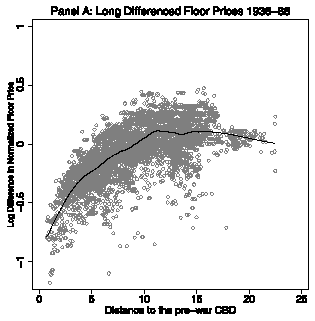
\includegraphics[height=0.76\textheight,width=\textwidth,keepaspectratio]{figures/figure3-a.pdf}
\end{frame}

\begin{frame}{Reunification, 1986--2006}

  \centering
  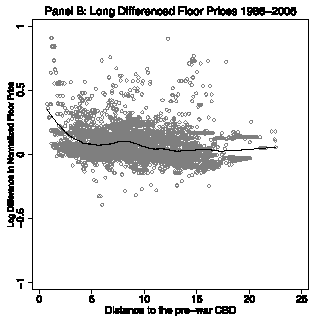
\includegraphics[height=0.76\textheight,width=\textwidth,keepaspectratio]{figures/figure3-b.pdf}
\end{frame}

\begin{frame}{Division, 1936--1966}

  \centering
  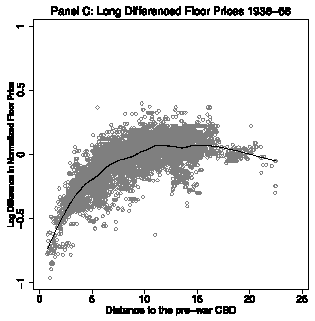
\includegraphics[height=0.76\textheight,width=\textwidth,keepaspectratio]{figures/figure3-c.pdf}
\end{frame}

\begin{frame}{Placebo, 1966--1986}

  \centering
  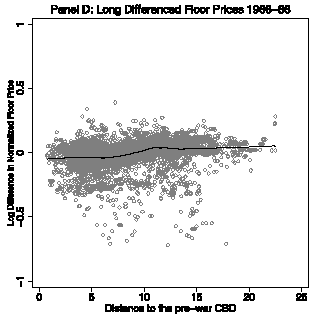
\includegraphics[height=0.76\textheight,width=\textwidth,keepaspectratio]{figures/figure3-d.pdf}
\end{frame}

\begin{frame}{Placebo, 1928--1936}

  \centering
  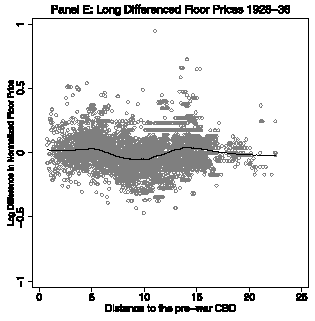
\includegraphics[height=0.76\textheight,width=\textwidth,keepaspectratio]{figures/figure3-e.pdf}
\end{frame}

\begin{frame}{Table 1: Division, 1936--1986}

  \centering
  \fontsize{8}{8}\selectfont
  \setlength{\tabcolsep}{5pt}
  \renewcommand{\arraystretch}{1.05}
  \resizebox*{\textwidth}{5.4cm}{%
  \begin{tabular}{@{}l*{9}{c}@{}}
  \toprule
 & (1) & (2) & (3) & (4) & (5) & (6) & (7) & (8) & (9) \\
 & $\Delta\ln Q$ & $\Delta\ln Q$ & $\Delta\ln Q$ & $\Delta\ln Q$ & $\Delta\ln Q$ & $\Delta\ln EmpR$ & $\Delta\ln EmpR$ & $\Delta\ln EmpW$ & $\Delta\ln EmpW$ \\
\midrule
CBD 1 & $-0.800^{***}$ & $-0.567^{***}$ & $-0.524^{***}$ & $-0.503^{***}$ & $-0.565^{***}$ & $-1.332^{***}$ & $-0.975^{***}$ & $-0.691^{*}$ & $-0.639^{*}$ \\
 & $(0.071)$ & $(0.071)$ & $(0.071)$ & $(0.071)$ & $(0.077)$ & $(0.383)$ & $(0.311)$ & $(0.408)$ & $(0.338)$ \\
CBD 2 & $-0.655^{***}$ & $-0.422^{***}$ & $-0.392^{***}$ & $-0.360^{***}$ & $-0.400^{***}$ & $-0.715^{**}$ & $-0.361$ & $-1.253^{***}$ & $-1.367^{***}$ \\
 & $(0.042)$ & $(0.047)$ & $(0.046)$ & $(0.043)$ & $(0.050)$ & $(0.299)$ & $(0.280)$ & $(0.293)$ & $(0.243)$ \\
CBD 3 & $-0.543^{***}$ & $-0.306^{***}$ & $-0.294^{***}$ & $-0.258^{***}$ & $-0.247^{***}$ & $-0.911^{***}$ & $-0.460^{**}$ & $-0.341$ & $-0.471^{**}$ \\
 & $(0.034)$ & $(0.039)$ & $(0.037)$ & $(0.032)$ & $(0.034)$ & $(0.239)$ & $(0.206)$ & $(0.241)$ & $(0.190)$ \\
CBD 4 & $-0.436^{***}$ & $-0.207^{***}$ & $-0.193^{***}$ & $-0.166^{***}$ & $-0.176^{***}$ & $-0.356^{**}$ & $-0.259$ & $-0.512^{***}$ & $-0.521^{***}$ \\
 & $(0.022)$ & $(0.033)$ & $(0.033)$ & $(0.030)$ & $(0.026)$ & $(0.145)$ & $(0.159)$ & $(0.199)$ & $(0.169)$ \\
CBD 5 & $-0.353^{***}$ & $-0.139^{***}$ & $-0.123^{***}$ & $-0.098^{***}$ & $-0.100^{***}$ & $-0.301^{***}$ & $-0.143$ & $-0.436^{***}$ & $-0.340^{***}$ \\
 & $(0.016)$ & $(0.024)$ & $(0.024)$ & $(0.023)$ & $(0.020)$ & $(0.110)$ & $(0.113)$ & $(0.151)$ & $(0.124)$ \\
CBD 6 & $-0.291^{***}$ & $-0.125^{***}$ & $-0.094^{***}$ & $-0.077^{***}$ & $-0.090^{***}$ & $-0.360^{***}$ & $-0.135$ & $-0.280^{**}$ & $-0.142$ \\
 & $(0.018)$ & $(0.019)$ & $(0.017)$ & $(0.016)$ & $(0.016)$ & $(0.100)$ & $(0.089)$ & $(0.130)$ & $(0.116)$ \\
\midrule
Inner Boundary 1--6 &  &  & Yes & Yes & Yes &  & Yes &  & Yes \\
Outer Boundary 1--6 &  &  & Yes & Yes & Yes &  & Yes &  & Yes \\
Kudamm 1--6 &  &  &  & Yes & Yes &  & Yes &  & Yes \\
Block Characteristics &  &  &  &  & Yes &  & Yes &  & Yes \\
District Fixed Effects &  & Yes & Yes & Yes & Yes & Yes & Yes & Yes & Yes \\
Observations & 6,260 & 6,260 & 6,260 & 6,260 & 6,260 & 5,978 & 5,978 & 2,844 & 2,844 \\
$R^2$ & 0.26 & 0.51 & 0.63 & 0.65 & 0.71 & 0.19 & 0.43 & 0.12 & 0.33 \\
\bottomrule
  \end{tabular}}
  \vspace{0.35em}
  \parbox{\textwidth}{\fontsize{5.5}{6.5}\selectfont
  $Q$: floor price. $EmpR$: employment by residence. $EmpW$: employment by workplace.
  CBD 1--6: six 500 m distance bands from the pre-war CBD.
  Inner/Outer Boundary and Kudamm: six 500 m distance bands from the respective boundary or Breitscheid Platz.
  Block characteristics: distances to schools, parks and water, block area, wartime destruction, land use,
  government buildings and urban regeneration policies.
  HAC standard errors (Conley, 1999) in parentheses.
  $^{*}p<0.10$, $^{**}p<0.05$, $^{***}p<0.01$.}
\end{frame}

\begin{frame}{Table 2: Reunification, 1986--2006}

  \centering
  \fontsize{8}{8}\selectfont
  \setlength{\tabcolsep}{5pt}
  \renewcommand{\arraystretch}{1.05}
  \resizebox*{\textwidth}{5.4cm}{%
  \begin{tabular}{@{}l*{9}{c}@{}}
  \toprule
 & (1) & (2) & (3) & (4) & (5) & (6) & (7) & (8) & (9) \\
 & $\Delta\ln Q$ & $\Delta\ln Q$ & $\Delta\ln Q$ & $\Delta\ln Q$ & $\Delta\ln Q$ & $\Delta\ln EmpR$ & $\Delta\ln EmpR$ & $\Delta\ln EmpW$ & $\Delta\ln EmpW$ \\
\midrule
CBD 1 & $0.398^{***}$ & $0.408^{***}$ & $0.368^{***}$ & $0.369^{***}$ & $0.281^{***}$ & $1.079^{***}$ & $1.025^{***}$ & $1.574^{***}$ & $1.249^{**}$ \\
 & $(0.105)$ & $(0.090)$ & $(0.083)$ & $(0.081)$ & $(0.088)$ & $(0.307)$ & $(0.297)$ & $(0.479)$ & $(0.517)$ \\
CBD 2 & $0.290^{***}$ & $0.289^{***}$ & $0.257^{***}$ & $0.258^{***}$ & $0.191^{**}$ & $0.589^{*}$ & $0.538^{*}$ & $0.684^{**}$ & $0.457$ \\
 & $(0.111)$ & $(0.096)$ & $(0.090)$ & $(0.088)$ & $(0.087)$ & $(0.315)$ & $(0.299)$ & $(0.326)$ & $(0.334)$ \\
CBD 3 & $0.122^{***}$ & $0.120^{***}$ & $0.110^{***}$ & $0.115^{***}$ & $0.063^{**}$ & $0.340^{*}$ & $0.305^{*}$ & $0.326$ & $0.158$ \\
 & $(0.037)$ & $(0.033)$ & $(0.032)$ & $(0.032)$ & $(0.028)$ & $(0.180)$ & $(0.158)$ & $(0.216)$ & $(0.239)$ \\
CBD 4 & $0.033^{***}$ & $0.031$ & $0.030$ & $0.034$ & $0.017$ & $0.110$ & $0.034$ & $0.336^{**}$ & $0.261$ \\
 & $(0.013)$ & $(0.023)$ & $(0.022)$ & $(0.021)$ & $(0.020)$ & $(0.068)$ & $(0.066)$ & $(0.161)$ & $(0.185)$ \\
CBD 5 & $0.025^{***}$ & $0.018$ & $0.020$ & $0.020$ & $0.015$ & $-0.012$ & $-0.056$ & $0.114$ & $0.066$ \\
 & $(0.010)$ & $(0.015)$ & $(0.014)$ & $(0.014)$ & $(0.013)$ & $(0.056)$ & $(0.057)$ & $(0.118)$ & $(0.131)$ \\
CBD 6 & $0.019^{**}$ & $-0.000$ & $-0.000$ & $-0.003$ & $0.005$ & $0.060$ & $0.053$ & $0.049$ & $0.110$ \\
 & $(0.009)$ & $(0.012)$ & $(0.012)$ & $(0.012)$ & $(0.011)$ & $(0.039)$ & $(0.041)$ & $(0.095)$ & $(0.098)$ \\
\midrule
Inner Boundary 1--6 &  &  & Yes & Yes & Yes &  & Yes &  & Yes \\
Outer Boundary 1--6 &  &  & Yes & Yes & Yes &  & Yes &  & Yes \\
Kudamm 1--6 &  &  &  & Yes & Yes &  & Yes &  & Yes \\
Block Characteristics &  &  &  &  & Yes &  & Yes &  & Yes \\
District Fixed Effects &  & Yes & Yes & Yes & Yes & Yes & Yes & Yes & Yes \\
Observations & 7,050 & 7,050 & 7,050 & 7,050 & 7,050 & 6,718 & 6,718 & 5,602 & 5,602 \\
$R^2$ & 0.08 & 0.32 & 0.34 & 0.35 & 0.43 & 0.04 & 0.07 & 0.03 & 0.06 \\
\bottomrule
  \end{tabular}}
  \vspace{0.35em}
  \parbox{\textwidth}{\fontsize{5.5}{6.5}\selectfont
  $Q$: floor price. $EmpR$: employment by residence. $EmpW$: employment by workplace.
  CBD 1--6: six 500 m distance bands from the pre-war CBD.
  Inner/Outer Boundary and Kudamm: six 500 m distance bands from the respective boundary or Breitscheid Platz.
  Block characteristics: distances to schools, parks and water, block area, wartime destruction, land use,
  government buildings and urban regeneration policies.
  HAC standard errors (Conley, 1999) in parentheses.
  $^{*}p<0.10$, $^{**}p<0.05$, $^{***}p<0.01$.}
\end{frame}


\section{Model: Workers}
\subsection{Workers}
\begin{frame}{Model: Workers}
\framesubtitle{Consumption Index}
\centering
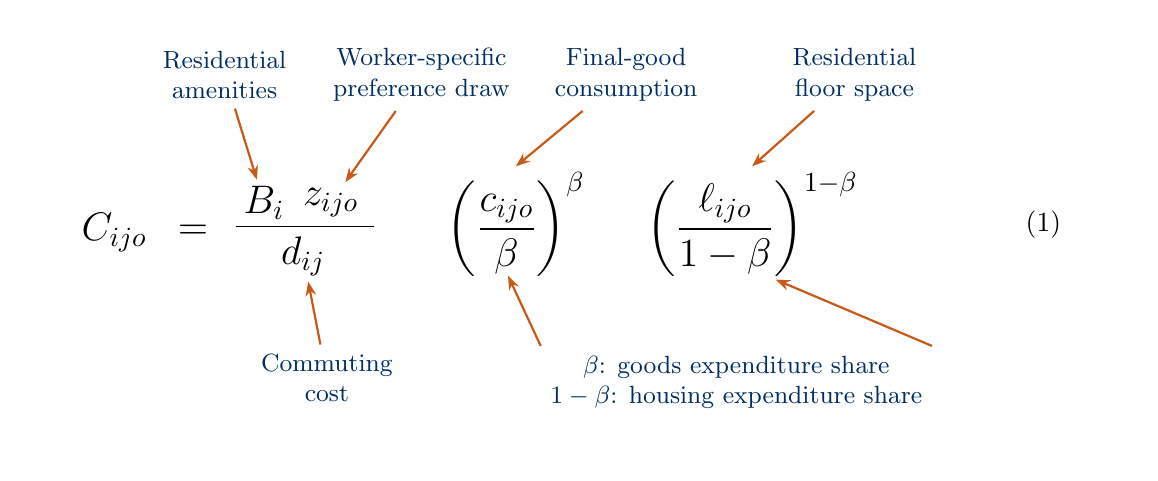
\begin{tikzpicture}[x=1cm,y=1cm]
  \path[use as bounding box] (0,0) rectangle (14,5.4);
  \node[term] (C) at (1.1,2.8) {$C_{ijo}$};
  \node[term] at (2.1,2.8) {$=$};
  \node[term] (B) at (3.0,3.18) {$B_i$};
  \node[term] (z) at (3.85,3.18) {$z_{ijo}$};
  \draw (2.65,2.87)--(4.4,2.87);
  \node[term] (d) at (3.5,2.5) {$d_{ij}$};
  \node[term] (c) at (6.2,2.9) {$\displaystyle\left(\frac{c_{ijo}}{\beta}\right)^\beta$};
  \node[term] (l) at (9.2,2.9) {$\displaystyle\left(\frac{\ell_{ijo}}{1-\beta}\right)^{1-\beta}$};
  \node at (12.9,2.9) {$(1)$};
  \node[lab] (lb) at (2.5,4.8) {Residential\\amenities};
  \node[lab] (lz) at (5.0,4.8) {Worker-specific\\preference draw};
  \node[lab] (ld) at (3.8,0.95) {Commuting\\cost};
  \node[lab] (lg) at (7.6,4.8) {Final-good\\consumption};
  \node[lab] (ll) at (10.5,4.8) {Residential\\floor space};
  \node[lab] (beta) at (9.0,0.9) {$\beta$: goods expenditure share\\$1-\beta$: housing expenditure share};
  \draw[arr] (lb)--(B); \draw[arr] (lz)--(z);
  \draw[arr] (ld)--(d); \draw[arr] (lg)--(c.north); \draw[arr] (ll)--(l.north);
  \draw[arr] (beta.north west)--(6.1,2.25);
  \draw[arr] (beta.north east)--(9.5,2.2);
\end{tikzpicture}
\par\small $i$: residence block \qquad $j$: workplace block \qquad $o$: worker
\end{frame}

\begin{frame}{Model: Workers}
\framesubtitle{Idiosyncratic Preferences}
\centering
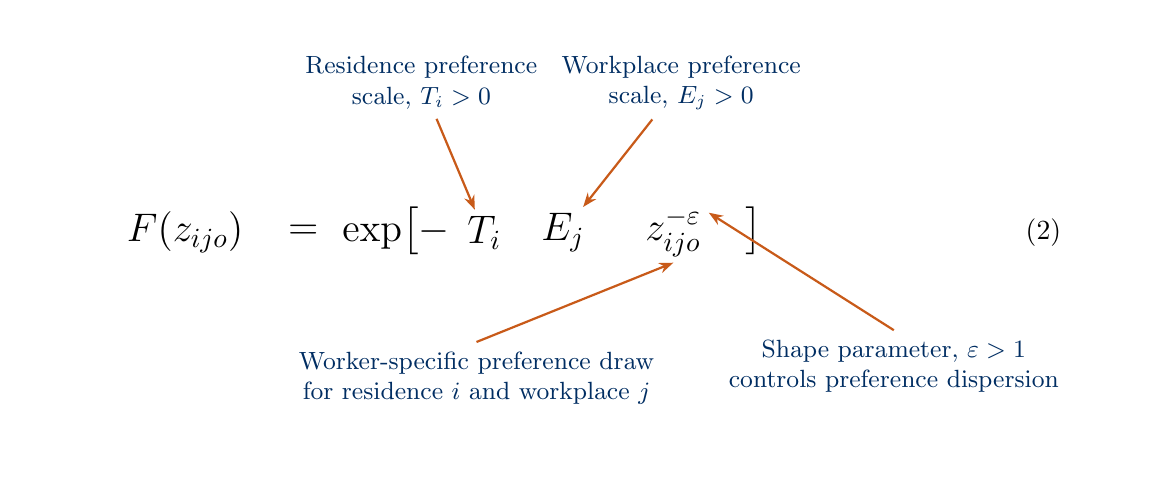
\begin{tikzpicture}[x=1cm,y=1cm]
  \path[use as bounding box] (0,0) rectangle (14,5.4);
  \node[term] (F) at (2.0,2.8) {$F(z_{ijo})$};
  \node[term] at (3.5,2.8) {$=$};
  \node[term] at (4.7,2.8) {$\exp\!\left[-\vphantom{z_{ijo}^{-\varepsilon}}\right.$};
  \node[term] (T) at (5.8,2.8) {$T_i$};
  \node[term] (E) at (6.8,2.8) {$E_j$};
  \node[term] (z) at (8.2,2.8) {$z_{ijo}^{-\varepsilon}$};
  \node[term] at (9.2,2.8) {$\left.\vphantom{z_{ijo}^{-\varepsilon}}\right]$};
  \node at (12.9,2.8) {$(2)$};
  \node[lab] (lT) at (5.0,4.7) {Residence preference\\scale, $T_i>0$};
  \node[lab] (lE) at (8.3,4.7) {Workplace preference\\scale, $E_j>0$};
  \node[lab] (lz) at (5.7,0.95) {Worker-specific preference draw\\for residence $i$ and workplace $j$};
  \node[lab] (leps) at (11.0,1.1) {Shape parameter, $\varepsilon>1$\\controls preference dispersion};
  \draw[arr] (lT)--(T);
  \draw[arr] (lE)--(E);
  \draw[arr] (lz.north)--(z.south);
  \draw[arr] (leps.north)--(8.65,3.05);
\end{tikzpicture}
\par\small Independent draws across residence--workplace pairs for each worker.
\end{frame}

\begin{frame}{Model: Workers}
\framesubtitle{Indirect Utility}
\centering
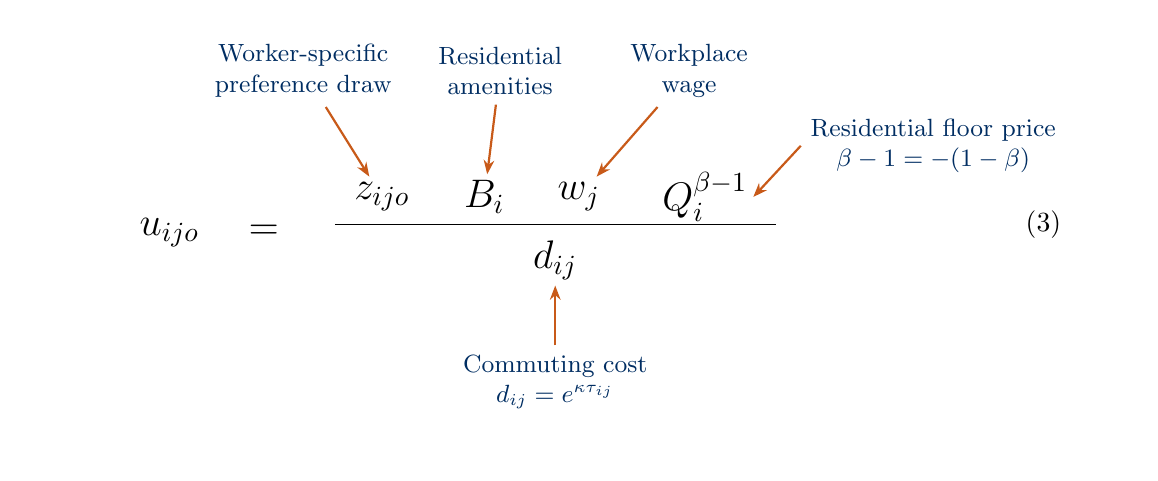
\begin{tikzpicture}[x=1cm,y=1cm]
  \path[use as bounding box] (0,0) rectangle (14,5.4);
  \node[term] (u) at (1.8,2.8) {$u_{ijo}$};
  \node[term] at (3.0,2.8) {$=$};
  \node[term] (z) at (4.5,3.25) {$z_{ijo}$};
  \node[term] (B) at (5.8,3.25) {$B_i$};
  \node[term] (w) at (7.0,3.25) {$w_j$};
  \node[term] (Q) at (8.6,3.25) {$Q_i^{\beta-1}$};
  \draw (3.9,2.9)--(9.5,2.9);
  \node[term] (d) at (6.7,2.45) {$d_{ij}$};
  \node at (12.9,2.9) {$(3)$};
  \node[lab] (lz) at (3.5,4.85) {Worker-specific\\preference draw};
  \node[lab] (lb) at (6.0,4.85) {Residential\\amenities};
  \node[lab] (lw) at (8.4,4.85) {Workplace\\wage};
  \node[lab] (lq) at (11.5,3.9) {Residential floor price\\$\beta-1=-(1-\beta)$};
  \node[lab] (ld) at (6.7,0.9) {Commuting cost\\$d_{ij}=e^{\kappa\tau_{ij}}$};
  \draw[arr] (lz)--(z); \draw[arr] (lb)--(B);
  \draw[arr] (lw)--(w); \draw[arr] (lq.west)--(Q.east); \draw[arr] (ld)--(d);
\end{tikzpicture}
\par\small $i$: residence \quad $j$: workplace \quad $o$: worker \qquad Final-good price normalised to 1
\end{frame}

\begin{frame}{Model: Workers}
\framesubtitle{Conditional Commuting Probability}
\centering
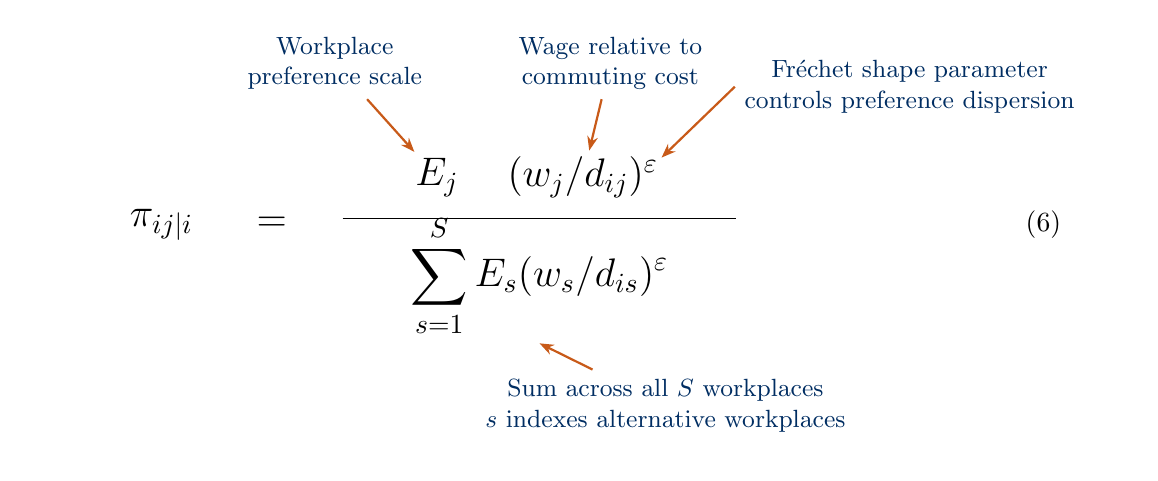
\begin{tikzpicture}[x=1cm,y=1cm]
  \path[use as bounding box] (0,0) rectangle (14,5.4);
  \node[term] (pi) at (1.7,2.9) {$\pi_{ij\mid i}$};
  \node[term] at (3.1,2.9) {$=$};
  \node[term] (E) at (5.2,3.5) {$E_j$};
  \node[term] (wd) at (7.05,3.5) {$(w_j/d_{ij})^\varepsilon$};
  \coordinate (eps) at (8.05,3.75);
  \draw (4.0,2.98)--(9.0,2.98);
  \node[term] (den) at (6.5,2.25) {$\displaystyle\sum_{s=1}^{S} E_s(w_s/d_{is})^\varepsilon$};
  \node at (12.9,2.9) {$(6)$};
  \node[lab] (le) at (3.9,4.95) {Workplace\\preference scale};
  \node[lab] (lwd) at (7.4,4.95) {Wage relative to\\commuting cost};
  \node[lab] (leps) at (11.2,4.65) {Fr\'echet shape parameter\\controls preference dispersion};
  \node[lab] (lden) at (8.1,0.6) {Sum across all $S$ workplaces\\$s$ indexes alternative workplaces};
  \draw[arr] (le)--(E); \draw[arr] (lwd)--(wd);
  \draw[arr] (leps.west)--(eps); \draw[arr] (lden)--(den.south);
\end{tikzpicture}
\par\small Given residence $i$, $Q_i$, $T_i$ and $B_i$ cancel from the choice probability.
\end{frame}

\section{Model: Production}
\begin{frame}{Model: Production}
\framesubtitle{Production Function}
\centering
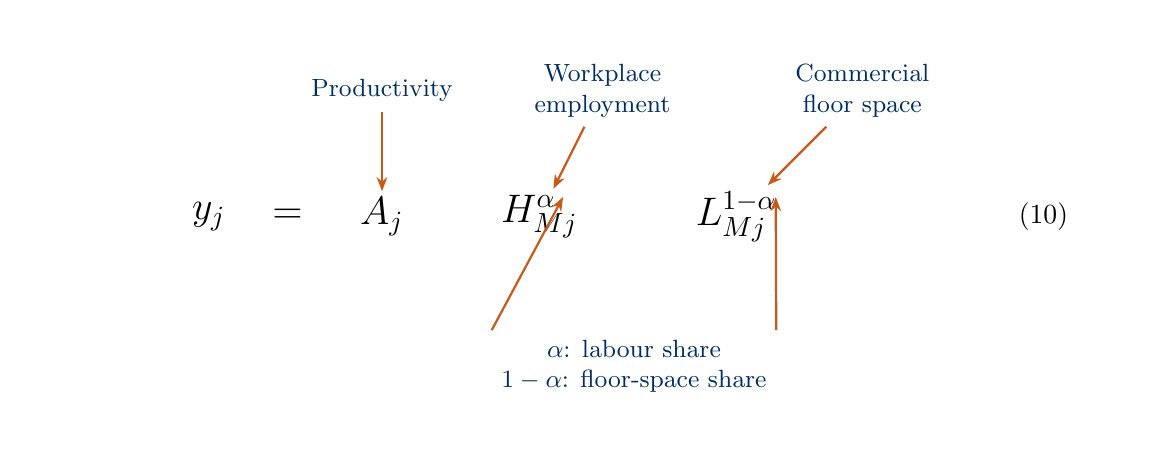
\begin{tikzpicture}[x=1cm,y=1cm]
  \path[use as bounding box] (0,0) rectangle (14,5.1);
  \node[term] (y) at (2.3,2.7) {$y_j$};
  \node[term] at (3.3,2.7) {$=$};
  \node[term] (A) at (4.5,2.7) {$A_j$};
  \node[term] (H) at (6.5,2.7) {$H_{Mj}^{\alpha}$};
  \node[term] (L) at (9.0,2.7) {$L_{Mj}^{1-\alpha}$};
  \node at (12.9,2.7) {$(10)$};
  \node[lab] (la) at (4.5,4.3) {Productivity};
  \node[lab] (lh) at (7.3,4.3) {Workplace\\employment};
  \node[lab] (ll) at (10.6,4.3) {Commercial\\floor space};
  \node[lab] (alpha) at (7.7,0.8) {$\alpha$: labour share\\$1-\alpha$: floor-space share};
  \draw[arr] (la)--(A);
  \draw[arr] (lh)--(H); \draw[arr] (ll)--(L);
  \draw[arr] (alpha.north west)--(6.8,2.95);
  \draw[arr] (alpha.north east)--(9.5,2.95);
\end{tikzpicture}
\par\small Perfect competition and constant returns to scale.
\end{frame}


\begin{frame}{Model: Production}
\framesubtitle{Employment}
\centering
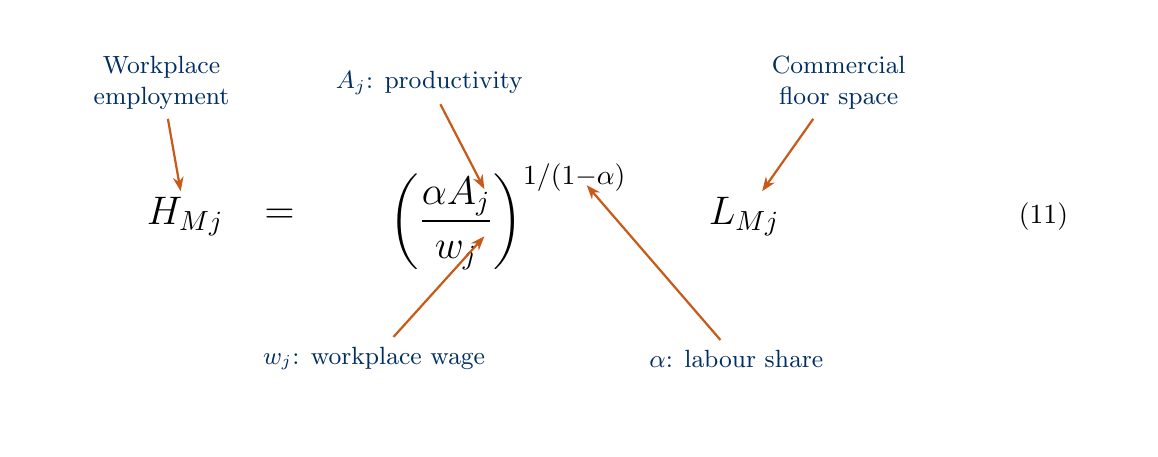
\begin{tikzpicture}[x=1cm,y=1cm]
  \path[use as bounding box] (0,0) rectangle (14,5.1);
  \node[term] (H) at (2,2.7) {$H_{Mj}$};
  \node[term] at (3.2,2.7) {$=$};
  \node[term] (ratio) at (6.1,2.7)
    {$\displaystyle\left(\frac{\alpha A_j}{w_j}\right)^{1/(1-\alpha)}$};
  \node[term] (L) at (9.1,2.7) {$L_{Mj}$};
  \node at (12.9,2.7) {$(11)$};
  \node[lab] (lh) at (1.7,4.4) {Workplace\\employment};
  \node[lab] (la) at (5.1,4.4) {$A_j$: productivity};
  \node[lab] (ll) at (10.3,4.4) {Commercial\\floor space};
  \node[lab] (lw) at (4.4,0.9) {$w_j$: workplace wage};
  \node[lab] (ls) at (9.0,0.9) {$\alpha$: labour share};
  \draw[arr] (lh)--(H); \draw[arr] (la)--(5.8,3.05);
  \draw[arr] (ll)--(L); \draw[arr] (lw)--(5.8,2.45);
  \draw[arr] (ls)--(7.1,3.1);
\end{tikzpicture}
\par\small Wages equate labour demand and commuting supply.
\end{frame}

\section{Model: Agglomeration}
\begin{frame}{Model: Agglomeration}
\centering
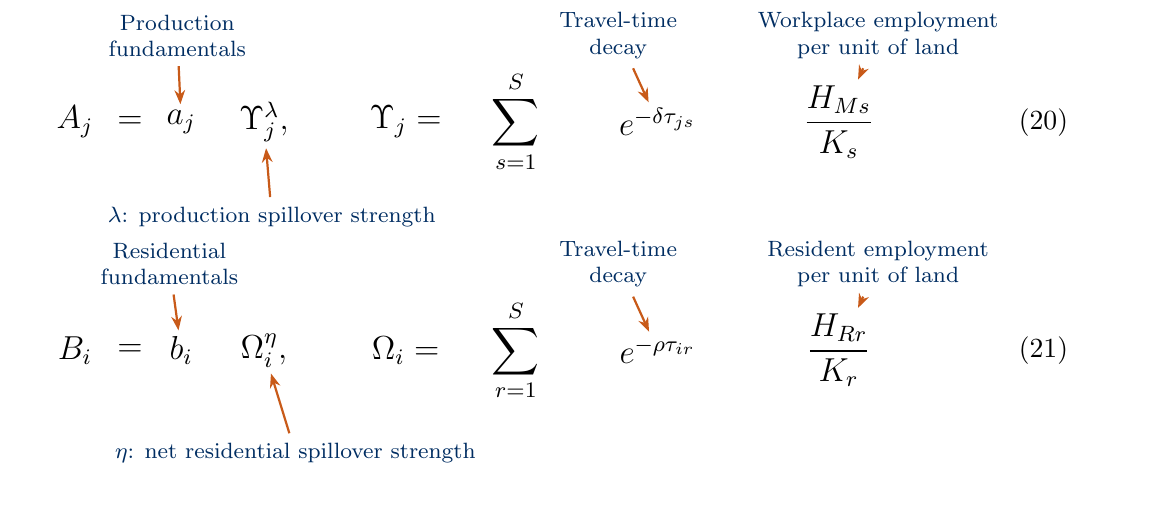
\begin{tikzpicture}[x=1cm,y=1cm,lab/.append style={font=\footnotesize},
  term/.append style={font=\large}]
  \path[use as bounding box] (0,0) rectangle (14,5.8);
  \node[term] (A) at (0.6,4.6) {$A_j$};
  \node[term] at (1.3,4.6) {$=$};
  \node[term] (a) at (1.95,4.6) {$a_j$};
  \node[term] (U) at (3.0,4.6) {$\Upsilon_j^\lambda,$};
  \node[term] at (4.8,4.6) {$\Upsilon_j=$};
  \node[term] at (6.2,4.6) {$\displaystyle\sum_{s=1}^{S}$};
  \node[term] (decay) at (8.0,4.6) {$e^{-\delta\tau_{js}}$};
  \node[term] (density) at (10.3,4.6) {$\displaystyle\frac{H_{Ms}}{K_s}$};
  \node at (12.9,4.6) {$(20)$};
  \node[lab] (la) at (1.9,5.7) {Production\\fundamentals};
  \node[lab] (ldecay) at (7.5,5.7) {Travel-time\\decay};
  \node[lab] (ldensity) at (10.8,5.7) {Workplace employment\\per unit of land};
  \node[lab] (lU) at (3.1,3.4) {$\lambda$: production spillover strength};
  \draw[arr] (la)--(a); \draw[arr] (ldecay)--(decay);
  \draw[arr] (ldensity)--(density); \draw[arr] (lU)--(U);
  \node[term] (B) at (0.6,1.7) {$B_i$};
  \node[term] at (1.3,1.7) {$=$};
  \node[term] (b) at (1.95,1.7) {$b_i$};
  \node[term] (O) at (3.0,1.7) {$\Omega_i^\eta,$};
  \node[term] at (4.8,1.7) {$\Omega_i=$};
  \node[term] at (6.2,1.7) {$\displaystyle\sum_{r=1}^{S}$};
  \node[term] (rdecay) at (8.0,1.7) {$e^{-\rho\tau_{ir}}$};
  \node[term] (rdensity) at (10.3,1.7) {$\displaystyle\frac{H_{Rr}}{K_r}$};
  \node at (12.9,1.7) {$(21)$};
  \node[lab] (lb) at (1.8,2.8) {Residential\\fundamentals};
  \node[lab] (lrdecay) at (7.5,2.8) {Travel-time\\decay};
  \node[lab] (lrdensity) at (10.8,2.8) {Resident employment\\per unit of land};
  \node[lab] (lO) at (3.4,0.4) {$\eta$: net residential spillover strength};
  \draw[arr] (lb)--(b); \draw[arr] (lrdecay)--(rdecay);
  \draw[arr] (lrdensity)--(rdensity); \draw[arr] (lO)--(O);
\end{tikzpicture}
\par\small $A_j$: productivity \quad $B_i$: amenities \quad
$\delta,\rho$: decay rates \quad $\tau$: travel time
\end{frame}

\section{Model: Solution}
\begin{frame}{Model: Solution}
  \small
  Given parameters and observed floor prices, workplace and residence
  employment, land area, and travel times:
  \vspace{0.5em}
  \begin{enumerate}
    \setlength{\itemsep}{0.7em}
    \item<1-> \textbf{Recover adjusted wages $\widetilde w$.}\\
      Match commuting flows to observed workplace and residence employment.
    \item<2-> \textbf{Recover adjusted productivity $\widetilde A$.}\\
      Use adjusted wages, floor prices and firms' zero-profit condition.
    \item<3-> \textbf{Recover adjusted amenities $\widetilde B$.}\\
      Use adjusted wages, floor prices, residence shares and population mobility.
    \item<4-> \textbf{Separate fundamentals from spillovers.}\\
      Apply (20)--(21):
      $\widetilde a_j=\widetilde A_j/\Upsilon_j^\lambda$ and
      $\widetilde b_i=\widetilde B_i/\Omega_i^\eta$.
    \item<5-> \textbf{Recover adjusted development density $\widetilde\phi$.}\\
      Use land area and implied floor-space demands to clear the land market.
  \end{enumerate}
  \vspace{0.5em}
\end{frame}


\begin{frame}{Model: Estimation}
  \large
  Estimation is by GMM using the Wall as exogenous variation.
  \vspace{1.5em}

  I'm going to skip this.
\end{frame}

\decksection{Model: Results}
\begin{frame}{Model: Results}
\framesubtitle{Table 5, column 3: pooled division and reunification estimates}
  \small
  \renewcommand{\arraystretch}{1.35}
  \begin{tabular}{@{}p{1.5cm}p{1.9cm}p{10.2cm}@{}}
    \toprule
    Parameter & Estimate (SE) & Meaning \\
    \midrule
    $\nu=\kappa\varepsilon$ & \shortstack{$0.0987^{***}$\\$(0.0016)$} & How quickly commuting flows decline as travel time rises. \\[0.5em]
    $\varepsilon$ & \shortstack{$6.6941^{***}$\\$(0.0934)$} & How similar workers' location preferences are. Higher values mean less dispersion. \\[0.5em]
    $\lambda$ & \shortstack{$0.0710^{***}$\\$(0.0054)$} & A 1\% rise in weighted workplace density raises productivity by 0.071\%. \\[0.5em]
    $\delta$ & \shortstack{$0.3617^{***}$\\$(0.0782)$} & How quickly production spillovers fade with travel time. \\[0.5em]
    $\eta$ & \shortstack{$0.1553^{***}$\\$(0.0083)$} & A 1\% rise in weighted resident density raises amenities by 0.155\%. \\[0.5em]
    $\rho$ & \shortstack{$0.7595^{***}$\\$(0.1741)$} & How quickly residential spillovers fade with travel time. \\
    \bottomrule
  \end{tabular}
  \par\vspace{0.4em}\scriptsize HAC standard errors in parentheses.
  $^{***}$ significant at 1\%. Travel time is measured in minutes.
\end{frame}

\begin{frame}{Model: Results}
\framesubtitle{Table 6: externalities and commuting costs}
  \centering
  \small
  \renewcommand{\arraystretch}{1.2}
  \begin{tabular}{@{}lccc@{}}
    \toprule
    Travel time & Production & Residential & Utility after \\
                & externalities & externalities & commuting \\
                & $e^{-\delta\tau}$ & $e^{-\rho\tau}$ & $e^{-\kappa\tau}$ \\
    \midrule
    0 minutes  & 1.000 & 1.000 & 1.000 \\
    1 minute   & 0.696 & 0.468 & 0.985 \\
    2 minutes  & 0.485 & 0.219 & 0.971 \\
    3 minutes  & 0.338 & 0.102 & 0.957 \\
    5 minutes  & 0.164 & 0.022 & 0.929 \\
    7 minutes  & 0.079 & 0.005 & 0.902 \\
    10 minutes & 0.027 & 0.001 & 0.863 \\
    15 minutes & 0.004 & 0.000 & 0.802 \\
    20 minutes & 0.001 & 0.000 & 0.745 \\
    30 minutes & 0.000 & 0.000 & 0.642 \\
    \bottomrule
  \end{tabular}
  \par\vspace{0.7em}
  Spillovers are highly local. Commuting utility declines much more slowly.
  \par\vspace{0.3em}\scriptsize
  Pooled estimates: $\delta=0.3617$, $\rho=0.7595$, $\kappa=0.0148$.
  Entries are remaining weights relative to zero travel time, rounded to three decimals.
\end{frame}

\begin{frame}{Model: Results}
\framesubtitle{Table 7: simulated versus observed}
  \centering
  \renewcommand{\arraystretch}{1.65}
  \setlength{\tabcolsep}{12pt}
  \begin{tabular}{@{}lrrrr@{}}
    \toprule
      & \multicolumn{2}{c}{Division} & \multicolumn{2}{c}{Reunification} \\
    \cmidrule(lr){2-3}\cmidrule(l){4-5}
    Distance band & Observed & Simulated & Observed & Simulated \\
    \midrule
    CBD 1 (nearest) & $-0.800$ & $-0.836$ & $0.398$ & $0.363$ \\
    CBD 3           & $-0.543$ & $-0.455$ & $0.122$ & $0.163$ \\
    CBD 6           & $-0.291$ & $-0.349$ & $0.019$ & $0.100$ \\
    \bottomrule
  \end{tabular}
  \par\vspace{0.8em}\small
  Effects on log floor prices in selected 500 m distance bands.\\
  Simulations use the baseline model with both spillovers.
\end{frame}

\begin{frame}{Extensions of the Framework}
  \small
  \begin{itemize}
    \setlength{\itemsep}{0.55em}
    \item \textbf{Monte, Redding and Rossi-Hansberg (2018), AER}\\
      \href{https://doi.org/10.1257/aer.20151507}{\emph{Commuting, Migration, and Local Employment Elasticities}}\\
      Brings in more complex labour market structure and studies local shocks.
    \item \textbf{Heblich, Redding and Sturm (2020), QJE}\\
      \href{https://doi.org/10.1093/qje/qjaa014}{\emph{The Making of the Modern Metropolis: Evidence from London}}\\
      Uses a QSM to study the rollout of railways in Victorian London
    \item \textbf{Couture, Gaubert, Handbury and Hurst (2024), REStud}\\
      \href{https://doi.org/10.1093/restud/rdad048}{\emph{Income Growth and the Distributional Effects of Urban Spatial Sorting}}\\
      Adds income heterogeneity and endogenous amenities.
    \item \textbf{Tsivanidis (2026), AER}\\
      \href{https://doi.org/10.1257/aer.20190874}{\emph{Evaluating the Impact of Urban Transit Infrastructure:
      Evidence from Bogot\'a's TransMilenio}}\\
      Adds worker groups and transit modes to evaluate welfare and distribution.
    \item \textbf{Robert-Nicoud, Combes, Duranton \& Gobillon, Working Paper out a week ago }\\
      \href{https://www.dropbox.com/scl/fi/q68a2vee7pke53zjl3f27/PIGLUM_live.pdf?rlkey=727pufl3n91drp7rbdqnk5p6p&e=1&dl=0}{\emph{A Unified Urban Model with Non-Homothetic Housing Demand}}\\
      Brings in more realistic housing demand which explains varying income shares spent on housing and the distribution of city sizes. 
  \end{itemize}
\end{frame}

\end{document}





